\documentclass[conference,a4paper]{IEEEtran}
\usepackage[T1]{fontenc}
\usepackage{graphicx,amsmath,amssymb,booktabs,array,multirow,balance}
\setlength{\tabcolsep}{3pt}
\usepackage{tikz}
\usetikzlibrary{arrows.meta,positioning,shapes.geometric,fit,calc}
\usepackage[hidelinks]{hyperref}
\hypersetup{pdftitle={Programmable Scan-Shift Activity Control in a MIPS32-Based Logic Built-In Self-Test Architecture},
pdfauthor={Gaurav Tiwari; Nishi Kumari; M.S.S.Harshitha},
pdfsubject={VL405 Design for Testability Lab project report},
pdfkeywords={LBIST, MIPS32, VHDL, scan chains, switching activity}}
\usepackage{url}
\graphicspath{{figures/}}
\newcommand{\rtl}[1]{\texttt{\detokenize{#1}}}
\newcommand{\figone}[4]{\begin{figure}[!t]\centering\includegraphics[width=\columnwidth]{#1}\caption{#2}\label{#3}\end{figure}#4}
\hyphenation{pseudo-random micro-architecture}
\title{Programmable Scan-Shift Activity Control in a\\MIPS32-Based Logic Built-In Self-Test Architecture}
% Shared affiliation and symbol-linked roll numbers, matching the reference.
\author{
\IEEEauthorblockN{
Gaurav Tiwari\textsuperscript{*}\quad
Nishi Kumari\textsuperscript{\(\dagger\)}\quad
M.S.S.Harshitha\textsuperscript{\(\ddagger\)}
}
\IEEEauthorblockA{
School of Computing and Electrical Engineering\\
Indian Institute of Technology Mandi, India\\
\textsuperscript{*}B24483,\quad
\textsuperscript{\(\dagger\)}B24495,\quad
\textsuperscript{\(\ddagger\)}B23272
}
}
\usepackage{listings}
\usepackage{xcolor}

% Include this file BEFORE \begin{document}.
\usepackage{listings}
\usepackage{xcolor}
\lstdefinestyle{projectvhdl}{
  language=VHDL,
  basicstyle=\ttfamily\scriptsize,
  keywordstyle=\color{blue!60!black},
  commentstyle=\color{green!35!black},
  stringstyle=\color{red!60!black},
  numbers=left,
  numberstyle=\tiny\color{gray},
  numbersep=5pt,
  breaklines=true,
  breakatwhitespace=false,
  columns=fullflexible,
  keepspaces=true,
  showstringspaces=false,
  tabsize=4,
  frame=single,
  captionpos=b,
  inputencoding=utf8,
  literate={–}{{-}}1 {─}{{-}}1 {×}{{$\times$}}1
}

\begin{document}
\maketitle

\begin{abstract}
Scan-based logic built-in self-test (LBIST) requires a controlled compromise
between switching activity, test application time, and fault observability.
This project implements a VHDL-2008 platform combining a single-cycle MIPS32
instruction-subset core, four balanced scan chains, a programmable
pseudorandom-pattern modifier, an eight-state LBIST controller, and a four-input
32-bit multiple-input signature register. The core exposes 1,024 architectural
state bits through four 256-cell chains. Rotating-priority transition suppression
reduces measured scan-input activity without inserting additional shift clocks.
For a four-pattern integrated experiment, the archived transition counts range
from 182 at the nominal 10\% setting to 2,057 in bypass over 4,096 lane-shift
opportunities, corresponding to 4.443\% and 50.220\% respectively. The repository
reports detection of all 2,048 injected scan-response fault configurations; this
result is explicitly restricted to the implemented observation-path model.
An activity-assumption sweep reports estimated dynamic power decreasing from
83 to 59 mW, while a separately archived routed-core implementation uses
2,430 LUTs and 1,024 flip-flops with +7.291 ns internal setup slack at 50 MHz.
The analysis distinguishes measured RTL activity, structural timing counts,
FPGA estimates, and unverified generalizations. It establishes a reproducible
integrated prototype while identifying the remaining requirements for exact
toggle-rate calibration and equal-coverage, activity-backed power validation.
\end{abstract}

\begin{IEEEkeywords}
logic built-in self-test, scan chains, MIPS32, pseudorandom patterns,
transition suppression, switching activity, VHDL, fault simulation
\end{IEEEkeywords}

\section{Introduction}
Logic built-in self-test integrates pattern generation, response collection,
and pass/fail decision logic around a circuit under test (CUT). In a scan-based
implementation, a test configuration is loaded serially into internal state,
a functional clock captures a response, and the response is shifted to a
compactor. The scan path provides controllability and observability, but
unconstrained patterns can cause substantial switching during repeated shifts.
Low-power scan-BIST research therefore treats the pattern stream and scan
application schedule as design variables rather than fixed overheads
\cite{gerstendorfer}.

The VL405 assignment asks for a scan-based LBIST architecture that modifies
embedded pseudorandom patterns to obtain a specified toggle rate without
sacrificing fault coverage or test time, using a MIPS32 architecture as the
example CUT. Its required deliverables are a VHDL hardware model, simulation
results, detailed performance analysis, and a project report \cite{assignment}.
The present report covers all three members' contributions and their final
integration, rather than treating the standalone modules as a finished system.

The implementation contributes (i) balanced access to the complete retained
state of an educational processor subset, (ii) programmable transition
suppression with fractional transition budgets, (iii) deterministic test
sequencing and parallel response compaction, and (iv) a source-traceable
evaluation separating activity, coverage, latency, and implementation cost.
The design and numerical results are anchored to repository revision
\rtl{bc81786} \cite{repository}. No new RTL modification or simulation campaign
is implied by preparation of this report.

\subsection{Assessment Against the Assignment}
The delivered hardware and test infrastructure satisfy the requirement for a
VHDL model and support the requested analyses. However, a programmable budget
is not equivalent to an arbitrary accurately achieved physical toggle rate.
Likewise, fixed controller cycle counts do not prove unchanged time to a
specified combinational-fault coverage. Accordingly, the report evaluates
these objectives individually and identifies where the available evidence
supports a result and where further experiments are needed.

\section{System Architecture and Integration}
\subsection{Functional Partition}
The integrated hierarchy is rooted at \rtl{lbist_mips32_top}. Member 1 supplies
the MIPS32-subset CUT, scan storage, partitioning, and chain-length analysis.
Member 2 supplies the LFSR, Hamming-distance logic, transition-budget controller,
pattern modifier, and standalone reference models. Member 3 supplies the LBIST
finite-state machine (FSM), MISR, signature comparison, and fault injector.
The final wrapper adds a 32-bit-to-four-lane adapter and an independent
scan-input activity monitor. Fig.~\ref{fig:architecture} summarizes the actual
data and control connections.

\begin{figure*}[!t]
\centering
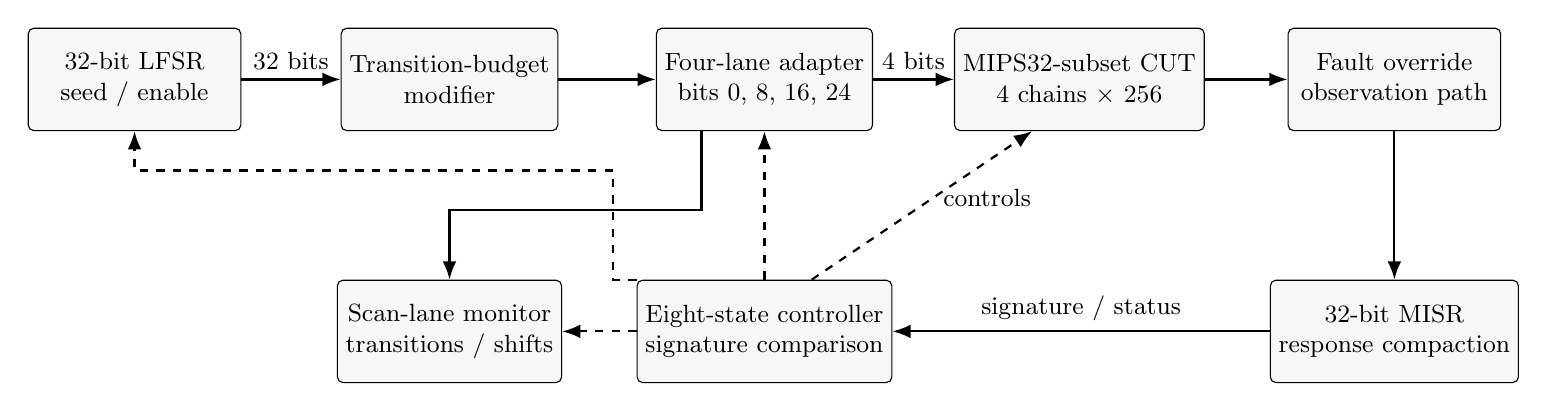
\begin{tikzpicture}[
  font=\small, >=Latex,
  box/.style={draw, rounded corners=2pt, align=center,
              minimum height=13mm, minimum width=27mm,
              fill=black!3, inner sep=3pt},
  data/.style={->, thick},
  ctrl/.style={->, thick, dashed}
]

% --- Layout constants (edit these two to rescale the whole figure) ---
\def\dx{4.0}   % horizontal pitch between top-row box centres
\def\dy{3.2}   % vertical distance between the two rows

% --- Top row: data path, left to right ---
\node[box] (prpg)  at (0*\dx, 0) {32-bit LFSR\\seed / enable};
\node[box] (mod)   at (1*\dx, 0) {Transition-budget\\modifier};
\node[box] (adapt) at (2*\dx, 0) {Four-lane adapter\\bits 0, 8, 16, 24};
\node[box] (core)  at (3*\dx, 0) {MIPS32-subset CUT\\4 chains $\times$ 256};
\node[box] (fault) at (4*\dx, 0) {Fault override\\observation path};

% --- Bottom row: monitor under modifier, FSM under adapter, MISR under fault override ---
\node[box] (monitor) at (1*\dx, -\dy) {Scan-lane monitor\\transitions / shifts};
\node[box] (fsm)     at (2*\dx, -\dy) {Eight-state controller\\signature comparison};
\node[box] (misr)    at (4*\dx, -\dy) {32-bit MISR\\response compaction};

% --- Top horizontal data arrows ---
\draw[data] (prpg)  -- node[above]{32 bits} (mod);
\draw[data] (mod)   -- (adapt);
\draw[data] (adapt) -- node[above]{4 bits} (core);
\draw[data] (core)  -- (fault);

% --- Right-side vertical data: fault override to MISR ---
\draw[data] (fault) -- (misr);

% --- Bottom horizontal data: MISR to FSM ---
\draw[data] (misr) -- node[above]{signature / status} (fsm);

% --- Adapter to monitor (solid; exits adapter's south offset-left so it clears the FSM-to-adapter vertical) ---
\draw[data] ([xshift=-8mm]adapt.south) -- ++(0, -10mm) -| (monitor.north);

% --- Dashed control signals from the controller ---
\draw[ctrl] (fsm.north) -- (adapt.south);                                   % FSM to adapter
\draw[ctrl] ([xshift=6mm]fsm.north)                                         % FSM to CUT
            -- node[right, pos=0.55]{controls}
            ([xshift=-6mm]core.south);
\draw[ctrl] (fsm.west) -- (monitor.east);                                   % FSM to monitor
\draw[ctrl] (fsm.north west) -- ++(-3mm, 0)                                 % FSM to LFSR (loopback)
            |- ([yshift=-5mm]prpg.south) -- (prpg.south);

\end{tikzpicture}
\caption{Integrated architecture reconstructed from the committed RTL. The
fault override lies after the CUT scan outputs; it does not modify the internal
CUT registers. The monitor observes four scan-input lanes rather than all
1,024 stored bits. Dashed arrows denote control connections.}
\label{fig:architecture}
\end{figure*}

\subsection{Integration Contracts}
All blocks use the rising edge of a common clock. The processor scan register
bank has active-high synchronous reset, whereas the PRPG, controller, and
activity monitor use active-low asynchronous system reset. The wrapper maps
\rtl{core_reset = dut_rst_sync or not rst_n}, allowing initialization to reset
the CUT at an active edge. The MISR has a separate active-low synchronous
reset asserted in the FSM's INIT state. Reset polarity is therefore translated
explicitly; it is not uniform across the hierarchy.

The PRPG enable is connected to \rtl{scan_enable}; its seed-load control is
asserted in INIT. The integrated stream consequently advances on each shift
edge and holds its sequential state in capture/idle intervals. The legacy
\rtl{prpg_advance} output is not the active PRPG handshake in the final wrapper.
Combinational outputs must still settle before the receiving edge. The
\rtl{pattern_valid} output is an enable indication, not a separately buffered
ready/valid protocol.

Instruction and load-data inputs remain external to the scan vector. The
integrated testbench fixes them to \rtl{0x24010001} (ADDIU r1,r0,1) and zero,
respectively. Thus, its captured workload is deterministic but does not
exercise the full implemented instruction set. In the integrated wrapper,
\rtl{run_enable} is tied low: it is a test harness around the processor, not
a complete processor boot-and-memory subsystem.

\section{MIPS32 CUT and Scan Architecture}
\subsection{Processor Scope}
The CUT is an original, single-cycle, 32-bit educational instruction subset.
Table~\ref{tab:isa} identifies its implemented operations. Register r0 is
hardwired to zero; arithmetic wraps where the unsigned instructions require
it. Signed and unsigned comparisons, sign-extended arithmetic immediates,
zero-extended logical immediates, branch offsets, and jump targets are decoded
in combinational next-state logic.

\begin{table}[!t]
\caption{Implemented Instruction Subset}
\label{tab:isa}\centering\small
\begin{tabular}{@{}p{.20\columnwidth}p{.73\columnwidth}@{}}\toprule
Class & Operations \\\midrule
Arithmetic & ADDU, SUBU, ADDIU, SLT, SLTU, SLTI, SLTIU \\
Logic & AND, OR, XOR, NOR, ANDI, ORI, XORI, LUI \\
Shift & SLL (including NOP), SRL, SRA \\
Memory & Word-aligned LW and SW \\
Control & BEQ, BNE, J, JAL, JR \\\bottomrule
\end{tabular}
\end{table}

There are no architectural delay slots; JAL writes PC+4. The design does not
implement exceptions, interrupts, HI/LO, multiplication/division, byte or
halfword accesses, caches, or privileged instructions. Unsupported operations
assert a diagnostic and advance the PC. Misaligned loads/stores are suppressed;
an unaligned JR reports an alignment diagnostic and falls through. These choices
make the CUT testable and compact but do not constitute full MIPS32 compliance.
Instruction and load reads are assumed combinational; synchronous FPGA block
RAM would require an adapter or a multicycle redesign.

\subsection{Architectural State and Scan Mapping}
The retained architectural state comprises
\begin{equation}
 B=32_{\mathrm{PC}}+31\times32_{\mathrm{GPR}}=1,024\;\mathrm{bits}.
\end{equation}
PC occupies state bits 31:0, and register $r$ occupies bits $32r+31:32r$ for
$1\leq r\leq31$. Excluding hardwired r0 avoids 32 unnecessary storage bits.
For $N$ chains, chain $c$ contains indices $c,c+N,c+2N,\ldots$, giving
\begin{equation}
 L_c=\left\lfloor\frac{B-1-c}{N}\right\rfloor+1,
 \qquad L_{\max}=\left\lceil\frac{B}{N}\right\rceil.
\label{eq:partition}
\end{equation}
The length difference is at most one. For $N=4$, every chain has 256 bits and
needs no padding or per-lane response mask. Input enters the lowest indexed
member and shifts toward the highest; scan output continuously exposes the
highest member. A desired vector must therefore be supplied in descending
position order on each chain. The full state-to-chain mapping is archived in
\rtl{scan_map_4chains.csv}.

Reset takes priority over shift; shift takes priority over functional capture;
otherwise the register bank holds its value. Functional execution uses
\rtl{run_enable}; test execution uses explicit scan/capture controls. Stores
to external memory are suppressed during reset, test mode, or run hold,
preventing a scan-loaded arbitrary register state from modifying memory.

\subsection{Partitioning Tradeoff}
Table~\ref{tab:chains} and Figs.~\ref{fig:lengths}--\ref{fig:latency} show the
calculated scan-length tradeoff. Four chains reduce full-load shift latency
from 1,024 to 256 clocks, an ideal $4\times$ shift speedup, at the cost of four
input and four output signals instead of one each. Three chains have lengths
342,341,341; a common 342-edge unload requires masking two invalid output slots.
The configurable scan bank supports such partitions, but the integrated LBIST
package is specifically configured for four equal chains.

\begin{table}[!t]\caption{Structural Scan-Partition Comparison}
\label{tab:chains}\centering\small
\begin{tabular}{@{}rrrrr@{}}\toprule
Chains & Min./max. length & Shift clocks & Shift+capture & I/O signals \\\midrule
1 & 1024/1024 & 1024 & 1025 & 2 \\
2 & 512/512 & 512 & 513 & 4 \\
3 & 341/342 & 342 & 343 & 6 \\
4 & 256/256 & 256 & 257 & 8 \\
8 & 128/128 & 128 & 129 & 16 \\
16 & 64/64 & 64 & 65 & 32 \\
32 & 32/32 & 32 & 33 & 64 \\\bottomrule
\end{tabular}
\end{table}
\figone{scan_chain_lengths.pdf}{Calculated maximum chain lengths for 1,024 state
bits. The four-chain default is highlighted.}{fig:lengths}{}
\figone{scan_latency_connectivity.pdf}{Calculated steady-state shift-plus-capture
latency and scan connectivity. These ideal counts exclude initialization,
FSM LOAD overhead, and final response drain.}{fig:latency}{}

Parallelism alone does not establish lower power: more lanes can switch at
once, and PRPG/MISR connections grow. The chosen four-chain configuration is a
balanced starting point, not a measured global optimum across area, routing,
energy, and coverage.

\section{Programmable Pattern Generation}
\subsection{LFSR and Four-Lane Adaptation}
The standalone Member-2 reference uses a 16-bit right-shifting Galois LFSR with
mask \rtl{0xB400} and default seed \rtl{0xACE1}. The integrated path sets
$W=32$, loads seed \rtl{0x1ACEB00C}, and uses a left-shift feedback recurrence
whose mask is \rtl{0x00200003}. The same tap positions are used in the MISR.
This report specifies the implemented recurrence rather than inferring a
maximal period from a polynomial comment; the integrated 32-bit sequence
period has not been established by the archived experiments.

Zero-seed loading selects an all-ones recovery seed. During enabled operation,
zero-state detection also selects a nonzero recovery state. The modified
32-bit vector drives four scan lanes through bit positions 0, 8, 16, and 24.
The standalone serial modifier output is not used by this integrated adapter.

\subsection{Rotating Transition Suppression}
Let $X_t$ denote the raw LFSR vector and $Y_{t-1}$ the previously accepted
modified vector. Requested transitions are
\begin{equation}
 D_t=X_t\oplus Y_{t-1}.
\end{equation}
A priority scan begins at offset $r_t$, grants at most $K_t$ requested
transitions, and rotates the grant vector back into the original bit positions.
For approved mask $A_t$,
\begin{equation}
 Y_t=Y_{t-1}\oplus A_t,\qquad
 \operatorname{popcount}(A_t)\leq K_t.
\label{eq:modifier}
\end{equation}
Unapproved bits retain their earlier value. Bypass instead forwards the raw
LFSR vector. Varying the starting priority reduces the fixed-lane preference
of a simple low-index priority encoder; it does not mathematically guarantee
equal excitation or equal fault detection across all logic cones.

\subsection{Budget Dithering and Mode Semantics}
The nominal mode codes select 10,20,30,40,50,60\%, bypass, or a custom integer
budget. The fractional accumulator alternates adjacent integer quotas; for
example, the 10\% mode averages 1.6 allowed transitions per 16-bit vector by
alternating limits 1 and 2. A separate serial grant accumulator permits or
holds a requested serial transition.

The distinction between \emph{allowed} and \emph{realized} activity is essential.
If fewer transitions are requested than the budget permits, the modifier does
not invent additional transitions to reach an exact percentage. Moreover,
the committed controller retains the 16-bit budget constants when instantiated
at $W=32$: averages of 1.6,3.2,4.8,6.4,8.0,9.6 allowed transitions are not
32-bit quotas of 10--60\%. This explains part of the approximately halved
integrated rate; sparse lane selection and finite deterministic streams also
affect the measured value.

Two further implementation boundaries matter when generalizing the design.
The rotation pointer is four bits and therefore visits 16 offsets even in the
32-bit path. The five-bit popcount signals cannot encode 32 simultaneous
transitions. The present experiments do not establish full-width fairness or
overflow-free statistics for every possible 32-bit input. Width-aware quota,
pointer, and counter sizing are therefore necessary for a fully scalable design.

\section{LBIST Control, Compaction, and Fault Model}
\subsection{Controller Sequence}
The Moore FSM has eight states: IDLE, INIT, SHIFT, CAPTURE, LOAD, COMPARE,
PASS, and FAIL. Its principal controls are summarized in
Table~\ref{tab:fsm}. INIT resets the CUT and MISR and loads the PRPG seed.
SHIFT lasts exactly 256 edges, accepting four scan bits and compacting four
outgoing bits per edge. CAPTURE performs one functional edge. LOAD is a
one-edge inter-pattern hold, followed by the next SHIFT; the final CAPTURE
goes directly to COMPARE. PASS/FAIL remains latched until reset.

\begin{table}[!t]\caption{Actual Integrated Control Schedule}
\label{tab:fsm}\centering\small
\begin{tabular}{@{}lcccl@{}}\toprule
State & Test & Shift & Capture & Action \\\midrule
IDLE & 0 & 0 & 0 & Wait for start \\
INIT & 1 & 0 & 0 & Reset CUT/MISR; seed PRPG \\
SHIFT & 1 & 1 & 0 & Advance stream; update MISR \\
CAPTURE & 1 & 0 & 1 & Capture CUT next state \\
LOAD & 1 & 0 & 0 & Inter-pattern hold \\
COMPARE & 1 & 0 & 0 & Compare signature \\
PASS & 0 & 0 & 0 & done=1, pass=1 \\
FAIL & 0 & 0 & 0 & done=1, pass=0 \\\bottomrule
\end{tabular}
\end{table}

For $P$ SHIFT/CAPTURE pairs of length $L$, active state dwell from INIT through
COMPARE is
\begin{equation}
 C_{\mathrm{FSM}}=1+PL+P+(P-1)+1=P(L+2)+1.
\label{eq:fsm}
\end{equation}
For $P=4$, $L=256$, this is 1,033 state-clock intervals, of which 1,024 are
shift and four are capture. Start-edge conventions, reset, and testbench waits
add to externally observed elapsed time. At the testbench's 10 ns period,
1,033 intervals represent 10.33 $\mu$s; at the separate 50 MHz implementation
target they represent 20.66 $\mu$s. These are calculated durations, not new
hardware measurements.

Changing the transition budget adds no state to this FSM, so a fixed-$P$
experiment has unchanged cycle count across settings. This does not prove
unchanged time to equal coverage. In an ideal fully observed overlapped scan
schedule, all $P$ captured responses require
\begin{equation}
 C_{\mathrm{ideal}}=(P+1)L+P
\label{eq:ideal}
\end{equation}
before reset/controller overhead. Equation~\eqref{eq:ideal} includes a final
response drain and must not be confused with the shorter implemented schedule.

\subsection{MISR Update and Observation Window}
The four-input, 32-bit MISR shifts left, conditionally XORs the old MSB into
positions 21,1,0, and then XORs the four response bits into positions 3:0.
With $S_t$ its state and $R_t$ the zero-extended response bus,
\begin{equation}
 S_{t+1}=(S_t\ll1)\oplus
 \big(S_t[31]\cdot\mathtt{0x00200003}\big)\oplus R_t.
\end{equation}
The seed is all ones and the MISR is enabled only in SHIFT. A fault-free run
first learns the golden signature; a reset and replay must reproduce it.
Changing seed, capture instruction, lane order, shift count, or target mode
requires a correspondingly regenerated golden reference.

The controller compacts the initial zero/reset unload as well as later
responses. Critically, the last CAPTURE is followed by COMPARE without a final
SHIFT. Its new response is therefore absent from the signature. Four capture
edges do not imply four fully unloaded functional responses; only the first
three captures are subsequently shifted out in the four-pattern run. This is
an observation-window limitation of the committed schedule, not an additional
unreported test result.

An often-used ideal aliasing estimate for a 32-bit compactor is $2^{-32}$,
approximately $2.33\times10^{-10}$, under a uniform independent syndrome
assumption. It is not a guaranteed probability for this deterministic stream,
nor does it establish excitation of faults that never affect an observed bit.

\subsection{Implemented Fault-Injection Model}
The injector is physically located in the model between CUT scan outputs and
MISR inputs. For selected chain $c$ and position $j$, it counts enabled shifts
and sets a persistent flag when the pre-edge counter reaches $L-1-j$. Once
set, the selected observed output is forced to SA0 or SA1 until reset. Other
chains pass through unchanged.

This implements a delayed, persistent \emph{observation-path override}. It
does not force the corresponding internal CUT scan-cell state or propagate
a defect through the processor's combinational logic. Consequently,
\begin{equation}
 F=4\times256\times2=2,048
\end{equation}
enumerates chain/site/polarity injection configurations, not all gate-level
stuck-at sites in a MIPS32 processor. Although the integration notes describe
an intermediate physical-cell model, the final RTL's actual override mechanism
governs the interpretation here.

\section{Verification Method and Evidence}
\subsection{Evidence Hierarchy}
The evaluation uses four distinct evidence classes: (i) calculated structural
counts, (ii) archived RTL experiment counts and supplied standalone results,
(iii) raw archived Vivado core reports, and (iv) an integrated power CSV whose
raw tool reports and sweep script are not included. This hierarchy prevents
an estimate or a handoff-level assertion from being presented as a measured
full-system result. Data and figure lineage is summarized in Appendix~A.

GHDL compilation uses VHDL-2008 and analyzes packages before dependent
entities \cite{ghdl}. Vivado behavioral simulation provides a separate
simulator check \cite{ug900}. The original processor regression covers every
implemented instruction kind, signed/unsigned behavior, r0, load/store buses,
branches/jumps, unsupported instructions, alignment diagnostics, run hold,
test hold, and scan load/capture/unload. The scan-bank regression compares an
independently updated vector model with the RTL after each edge for 1,024 bits
and 1,2,3,4,8,16,32 chains, plus 17-bit/3-chain and 1-bit/1-chain boundaries.
The archived log records ten passing simulation configurations and successful
GHDL synthesis elaboration. Its time-zero numeric\_std settling warning does
not persist during execution.

Member-2 tests cover quota bounds, bypass, standalone baseline measurement,
mode changes, reset behavior, and a 500-cycle lockup check in the committed
testbench. Its 32-cell reference model counts all model-cell transitions.
Member-3 tests cover MISR seed/hold behavior, FSM match/mismatch decisions,
control sequencing, and a four-chain placeholder harness. Placeholder-DUT
results are supporting unit tests, not measurements on the processor CUT.
The legacy scalar sweep bench also retains an older interface; it is not the
authoritative integrated campaign harness.

\subsection{Integrated Experiment Configuration}
The final integrated bench uses four patterns, four lanes, a 10 ns clock,
seed \rtl{0x1ACEB00C}, instruction \rtl{0x24010001}, and zero read data.
It asserts exactly $256P$ shift edges and $P$ capture edges, no shift/capture
overlap, deterministic fault-free signature replay, nonzero input activity,
and bounded displayed activity. The complete injection sweep selects all
four chains, all 256 positions, and both polarities, resetting between runs.
The default target code is 6 (bypass). Reduced-toggle activity runs disable
the fault loop and change the target-code generic.

The integrated campaign's assertion threshold is 90\%, whereas the repository
reports an observed 100\% result. A PASS message alone therefore does not prove
2,048/2,048 detection; the explicit detected/total counts are the relevant
coverage evidence. The coverage figure is generated from fixed 2,048 and zero
values in the plotting script, corroborating the documented result but not
constituting an independent machine-parsed fault log.

\section{Results and Performance Analysis}
\subsection{Integrated Scan-Input Activity}
The scan monitor compares consecutive input lane values only during SHIFT.
It clears its previous-valid flag outside SHIFT, so the first comparison of
each block is excluded from the numerator. The denominator nevertheless
includes every shift edge:
\begin{equation}
 \hat\alpha_{\mathrm{lane}}=\frac{T}{4PL},\qquad
 R_{\mathrm{display}}=\left\lfloor100\hat\alpha_{\mathrm{lane}}\right\rfloor.
\label{eq:activity}
\end{equation}
For four patterns, there are 4,096 denominator opportunities and 4,080 valid
within-block comparison opportunities. This convention is retained when
calculating the rates in Table~\ref{tab:activity}.

\begin{table}[!t]\caption{Integrated Activity: Archived Counts and Recomputed Ratios}
\label{tab:activity}\centering\small
\begin{tabular}{@{}lrrrr@{}}\toprule
Mode & Transitions & Rate (\%) & Display (\%) & Reduction (\%) \\\midrule
10\% & 182 & 4.443 & 4 & 91.152 \\
20\% & 405 & 9.888 & 9 & 80.311 \\
30\% & 610 & 14.893 & 14 & 70.345 \\
40\% & 811 & 19.800 & 19 & 60.574 \\
50\% & 995 & 24.292 & 24 & 51.629 \\
60\% & 1206 & 29.443 & 29 & 41.371 \\
Bypass & 2057 & 50.220 & 50 & 0.000 \\\bottomrule
\end{tabular}
\vspace{2pt}\parbox{\columnwidth}{\footnotesize All rates use $T/4096$; reduction is
$100(1-T/2057)$. These are lane-input activity results, not total-core power.}
\end{table}

Fig.~\ref{fig:activity} preserves the repository's integer-display rates.
The precise rates above are derived from the archived raw counts and are not
new simulation measurements. For example, 405/4096 is 9.888\%, although the
RTL displays 9\%. Bypass means unmodified PRPG passthrough; its nominal 100\%
label is not a claim that every input bit toggles every cycle.

\figone{integrated_scan_activity.pdf}{Repository integrated activity plot.
The measured bars are integer-truncated display percentages; bypass denotes
100\% passthrough, not 100\% measured toggling.}{fig:activity}{}

The lowest-budget mode reduces the observed count from 2,057 to 182, a
91.152\% count-based lane-activity reduction. It does not achieve an actual
10\% lane-toggle rate; it realizes 4.443\% under this configuration. The
system therefore demonstrates programmable suppression and monotonic mode
ordering, rather than exact arbitrary-target calibration.

\subsection{Switching Proxy and Numerical Precision}
The archived proxy script normalizes the \emph{integer displayed percentages}
against bypass, producing 8,18,28,38,48,58,100\% of bypass and reported
reductions of 92,82,72,62,52,42,0\%. Fig.~\ref{fig:proxy} shows those original
values. They are dimensionless, and their quantization differs from ratios
computed directly from transition counts. For the 10\% setting, $4/50=8\%$
and a 92\% reduction are display-derived; $182/2057=8.848\%$ and a 91.152\%
reduction are count-derived. Both conventions are disclosed rather than mixed.

\figone{integrated_power_proxy.pdf}{Archived activity proxy normalized from
integer display rates. It expresses scan-lane switching ratios, not watts;
the count-based ratios are given in Table~\ref{tab:activity}.}{fig:proxy}{}

A first-order dynamic-power relation is
\begin{equation}
 P_{\mathrm{dyn}}\propto\alpha C_{\mathrm{eff}}V^2 f,
\end{equation}
with any event-definition factor absorbed into $C_{\mathrm{eff}}$. If all
other quantities were held fixed, lowering activity would lower the affected
switching component. The four-lane monitor, however, does not measure clock
tree power, leakage, glitches, internal combinational switching, or all scan
flops. It must not be converted directly into a guaranteed chip-power reduction.

\subsection{Standalone PRPG Findings}
Table~\ref{tab:standalone} includes the Member-2 handoff's reference experiment
for completeness. It uses a 16-bit PRPG and a separate 32-cell scan model,
not the four-lane integrated CUT. Reported 10\% operation has 49.19\% baseline
cell activity and 7.38\% modified activity, a relative reduction of about
85\%. That is a switching reduction; the handoff's wording ``power reduction''
is not treated as a physical measurement.

\begin{table}[!t]\caption{Member-2 Standalone Reference Results (Handoff-Reported)}
\label{tab:standalone}\centering\small
\begin{tabular}{@{}lrrrr@{}}\toprule
Mode & Base word & Mod. word & Base scan & Mod. scan \\
 & \multicolumn{4}{c}{Toggle rate (\%)} \\\midrule
Bypass & 52.28 & 52.28 & 50.42 & 50.42 \\
10\% & 49.00 & 10.00 & 49.19 & 7.38 \\
20\% & 50.45 & 19.98 & 50.10 & 9.50 \\
30\% & 49.23 & 29.62 & 49.73 & 13.96 \\
40\% & 50.92 & 38.70 & 50.82 & 18.66 \\
50\% & 52.65 & 46.17 & 52.86 & 25.07 \\
60\% & 50.25 & 48.75 & 51.84 & 28.24 \\\bottomrule
\end{tabular}
\end{table}

The handoff additionally lists 82 LUTs, 57 flip-flops, a 1.84 ns critical
path, and a less-than-0.5\% overhead claim on a different target. No corresponding
raw synthesis reports are archived for that standalone block, and the
percentage denominator is not independently established. Those figures are
not used as validated integrated resource or frequency results. Similarly,
the committed long-run unit bench checks 500 cycles, so a handoff narrative
about a 5,000-cycle uniqueness experiment is not substituted for that test.

\subsection{Reported Fault-Campaign Result}
The repository's post-integration analysis reports 2,048 detected configurations
out of 2,048 with four patterns and the final injector, compared with an earlier
1,762/2,048 result under a different injection interpretation. The final
coverage plot is included as Fig.~\ref{fig:coverage}. This is 100\% detection
within the defined delayed-output-override model, with zero reported
undetected cases. It does not establish 100\% processor logic-fault coverage.

\figone{integrated_fault_coverage.pdf}{Repository-reported four-pattern
campaign: 2,048 detected injection configurations, zero undetected. The source
plot calls this a physical-cell model; inspection of the committed RTL shows
a delayed persistent scan-output override. This scope governs the claim.}{fig:coverage}{}

The default campaign uses bypass mode. The activity sweep separately tests
reduced-toggle settings with the fault loop disabled. Therefore, unchanged
coverage at each reduced-toggle mode is not demonstrated by these two
experiments taken together. A matched per-mode coverage matrix, with identical
seed, instruction workload, fault universe, and observation window, is required
to substantiate the assignment's ``without sacrificing fault coverage'' goal.

\subsection{Routed Core Implementation}
The archived Vivado 2023.2 implementation targets XC7Z020-CLG400-1 with a
20 ns clock in out-of-context mode. Table~\ref{tab:vivado} and
Fig.~\ref{fig:utilization} report actual archived implementation results for
\rtl{mips32_core}, not the complete integrated LBIST wrapper. Synthesis uses
2,442 LUTs; routing reduces the count to 2,430. All 1,024 state registers remain
flip-flops; no latches, block RAM, or DSPs are inferred.

\begin{table}[!t]\caption{Archived Vivado Results: Four-Chain Core Only}
\label{tab:vivado}\centering\small
\resizebox{\columnwidth}{!}{\begin{tabular}{@{}lr@{}}\toprule
Metric & Result \\\midrule
Target / clock & XC7Z020-CLG400-1 / 50 MHz \\
Routed LUTs / available & 2,430 / 53,200 (4.57\%) \\
Flip-flops / available & 1,024 / 106,400 (0.96\%) \\
Latch / BRAM / DSP count & 0 / 0 / 0 \\
Worst setup / hold slack & +7.291 / +0.119 ns \\
Total negative setup / hold slack & 0 / 0 ns \\
Worst setup data-path delay & 12.702 ns \\
XSim core / 4-chain / 3-chain checks & PASS / PASS / PASS \\
DRC errors / warnings & 0 / 1 \\\bottomrule
\end{tabular}}
\end{table}

\figone{vivado_utilization.pdf}{Routed utilization of the default four-chain
core. The PRPG, modifier, controller, MISR, and instrumentation are not included
in this archived implementation.}{fig:utilization}{}

The timing report lists zero unconstrained internal endpoints, but 73 inputs
without input delays and 1,126 outputs without output delays. HD.CLK\_SRC is
unset, leaving top-level clock-buffer skew/delay unspecified. The ZPS7-1 DRC
warning identifies the missing processing-system block in a standalone Zynq
IP design. Thus, internal timing passes at the assumed 50 MHz; external
memory/board timing closure, a complete Zynq system, and a usable bitstream
remain outside this run. A positive slack value is not a measured maximum
processor operating frequency.

\subsection{Power Estimates: Two Different Experiments}
The core-only routed report gives a vectorless estimate of 116 mW total:
13 mW dynamic and 103 mW device static, with medium confidence and no
simulation activity file. This is distinct from the integrated power CSV.

The latter records a same-netlist activity-assumption sweep attributed to
\rtl{lbist_mips32_top}: dynamic power decreases from 83 to 59 mW as the
assumed toggle setting decreases from 100 to 10\%; static power remains
92 mW. Table~\ref{tab:power} and Figs.~\ref{fig:power}--\ref{fig:reduction}
preserve these supplied results. The dynamic reduction is
\begin{equation}
 \Delta P_{\mathrm{dyn}}=100\frac{83-59}{83}=28.916\%,
\end{equation}
whereas total estimated power decreases from 175 to 151 mW, or 13.714\%.
The 28.9\% figure must therefore be labeled \emph{dynamic}, not total power.

\begin{table}[!t]\caption{Supplied Integrated Activity-Assumption Power Sweep}
\label{tab:power}\centering\small
\begin{tabular}{@{}rrrrr@{}}\toprule
Activity (\%) & Dynamic & Static & Total & Dyn. reduction (\%) \\
 & \multicolumn{3}{c}{Estimated power (mW)} & \\\midrule
100 & 83 & 92 & 175 & 0.00 \\
90 & 82 & 92 & 174 & 1.20 \\
80 & 80 & 92 & 172 & 3.61 \\
70 & 78 & 92 & 170 & 6.02 \\
60 & 76 & 92 & 168 & 8.43 \\
50 & 74 & 92 & 166 & 10.84 \\
40 & 71 & 92 & 163 & 14.46 \\
30 & 68 & 92 & 160 & 18.07 \\
20 & 64 & 92 & 156 & 22.89 \\
10 & 59 & 92 & 151 & 28.92 \\\bottomrule
\end{tabular}
\end{table}

\figone{vivado_activity_power.pdf}{Supplied integrated same-netlist power
estimate versus assumed switching activity. These assumptions are not the
measured four-lane rates of Table~\ref{tab:activity}.}{fig:power}{}
\figone{vivado_dynamic_power_reduction.pdf}{Dynamic-power reduction computed
from the supplied activity-assumption sweep. At 10\% assumed activity, the
28.9\% dynamic reduction corresponds to 13.7\% total estimated reduction.}{fig:reduction}{}

The integrated sweep's exact target constraints, annotated nets, implementation
stage, and raw power reports are not committed alongside the CSV. The included
Vivado Tcl script still implements the core-only top. Accordingly, these values
are reported as a supplied sensitivity study, not an independently reproducible
full-wrapper implementation. AMD distinguishes vectorless activity prediction
from simulation-activity-backed power analysis \cite{ug907}. No SAIF file or
physical rail measurement is provided here, and the assumed activity percentages
must not be identified directly with the modifier's mode codes or achieved
lane rates.

\section{Discussion, Limitations, and Improvements}
\subsection{What the Evidence Establishes}
The VHDL hierarchy integrates real scan-accessible processor state with all
three members' blocks. The four-chain partition is exactly balanced and
reduces shift latency relative to a single chain. The input activity data show
strong, monotonic suppression without adding scan cycles to a fixed-pattern
controller run. Core implementation reports establish FPGA feasibility under
the documented internal timing assumptions. The reported fault campaign
validates signature discrimination over its defined injection configurations.

These findings meet substantial parts of the assignment, but they do not
justify an unrestricted statement that arbitrary exact scan power is achieved
with unchanged processor fault coverage and equal-coverage test time.
Table~\ref{tab:requirements} maps each deliverable to its evidence and scope.

\begin{table*}[!t]\caption{Assignment Requirements, Delivered Evidence, and Boundaries}
\label{tab:requirements}\centering\small
\begin{tabular}{@{}p{.22\textwidth}p{.39\textwidth}p{.33\textwidth}@{}}\toprule
Requirement & Delivered evidence & Boundary / remaining validation \\\midrule
VHDL hardware model & Processor subset, scan bank, LFSR/modifier, controller, MISR, injector, integrated wrapper & Educational ISA subset; external memories are not included \\
Simulation results & Core/scan logs, unit benches, integrated signature/protocol checks, activity CSV, documented fault sweep & Integrated raw full campaign log is not archived; placeholder results are separate \\
Detailed performance analysis & Chain-length/clock counts, transition rates, switching ratios, coverage, routed core timing/utilization, supplied power sensitivity & Lane activity is not all-flop/whole-chip activity; full-wrapper implementation not archived \\
Specified toggle rate / power & Six selectable budgets, custom mode, monotonic integrated suppression & 16-bit quotas retained at width 32; exact lane-rate calibration and activity-backed watts remain open \\
No coverage/test-time sacrifice & Same FSM schedule across modes; reported 2,048-case bypass campaign & Need equal-observation, per-mode gate-level coverage and time-to-coverage comparisons \\\bottomrule
\end{tabular}
\end{table*}

\subsection{Priority Improvements}
First, generate transition quotas from the actual width and selected target,
resize the rotation pointer to $\lceil\log_2 W\rceil$, and resize popcounts to
$\lceil\log_2(W+1)\rceil$. Calibrate the four selected lanes explicitly rather
than inferring their rates from the internal word budget. A closed-loop
lane-activity controller could track a specified measured rate, subject to
the excitation constraints of the available stream.

Second, mask the initial nonresponse unload and add a final response-drain
phase, so every requested capture contributes to the signature. Document
first/last edge conventions and regenerate the golden reference after changing
the observation schedule. Use larger workloads that exercise arithmetic,
memory, and control cones rather than one fixed ADDIU instruction.

Third, inject faults into internal scan state or a technology-mapped CUT
netlist, with independent fault-free and faulty propagation. Sweep each
target mode and multiple seeds at matched pattern budgets and then compare
time to the same coverage. The present 2,048 configuration count should remain
separate from any future gate-level fault universe.

Finally, archive a full-wrapper synthesis/implementation script, raw activity
logs, per-fault outcomes, and power reports. Annotate representative scan and
capture activity using SAIF/VCD, constrain external interfaces, and measure
board rails if physical power is required. Separate average shift power,
capture peaks, whole-test energy, and clock/control overhead. A lower input
transition count is useful evidence, but alone cannot quantify all of them.
\begin{figure*}[!t]
    \centering
    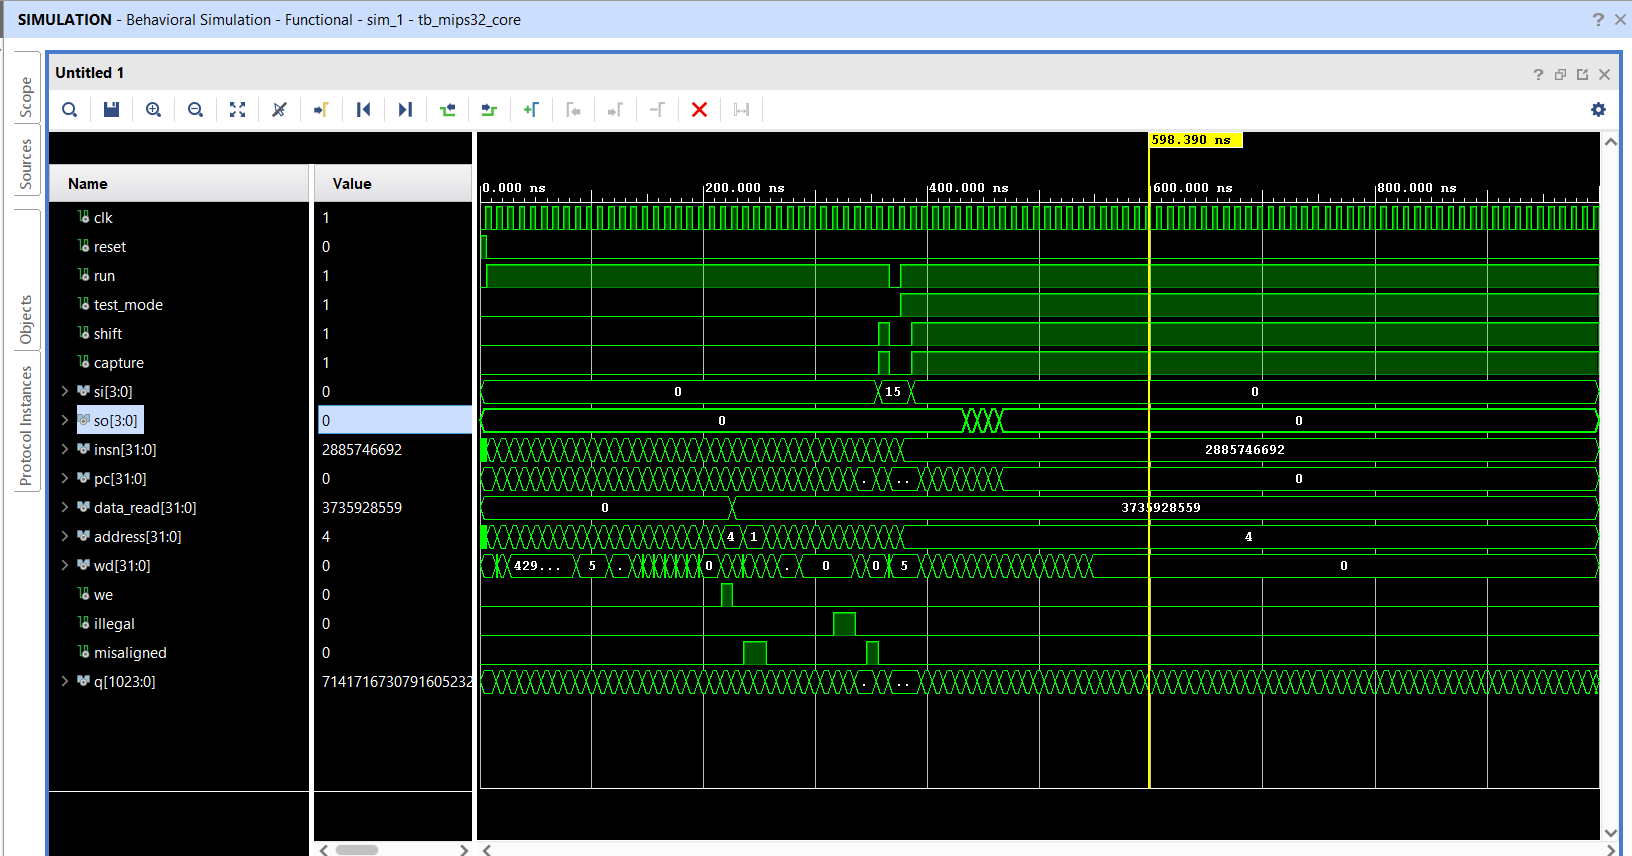
\includegraphics[width=\textwidth]
        {image.png}
    \caption{Vivado behavioral simulation of the MIPS32
    instruction-subset core, showing clock, reset,
    instruction input, program counter, and scan-control
    signals during functional execution and scan testing.}
    \label{fig:mips_core_waveform}
\end{figure*}

\section{Conclusion}
This project delivers a modular VHDL scan-based LBIST prototype integrating
a MIPS32-subset core, four balanced 256-cell chains, programmable transition
suppression, deterministic control, and parallel signature compaction. The
four-chain design provides a calculated $4\times$ shift-latency improvement
over a single chain. Archived integrated counts show input-lane activity
falling from 50.220\% in bypass to 4.443\% at the nominal 10\% budget, a
91.152\% count-based reduction. The repository reports all 2,048 injected
observation-path configurations detected in its bypass campaign. Separately,
the routed core meets its constrained internal timing target at 50 MHz using
2,430 LUTs and 1,024 flip-flops, and the supplied power sensitivity study shows
a 28.916\% estimated dynamic reduction under reduced assumed activity.
These results demonstrate the integration and the practical value of
programmable scan activity control. Exact target calibration, complete capture
observation, per-mode internal-logic fault coverage, and activity-backed
full-system power are the remaining steps toward the assignment's strongest
equal-coverage and equal-test-time claim.

\balance
\appendices
\section{Reproducibility and Evidence Map}
The source snapshot is \rtl{bc81786}; the report package includes an evidence
manifest of file hashes and report-generation notes. The analysis gives final
RTL precedence over historical handoff descriptions. All eight project result
figures are reused with captions that identify their data source and scope.
No plotted curve is represented as a new simulation run.

\begin{table}[!t]\caption{Primary Local Evidence}
\centering\footnotesize
\begin{tabular}{@{}p{.51\columnwidth}p{.43\columnwidth}@{}}\toprule
Repository location & Report use \\\midrule
\rtl{rtl/mips32_core.vhd}, scan bank/package & CUT semantics, state and chain mapping \\
\rtl{rtl/member2/} & PRPG, quotas, modifier and adapter \\
\rtl{rtl/member3/} & FSM, MISR and fault mechanism \\
\rtl{rtl/lbist_mips32_top.vhd} & Integrated handshake/reset mapping \\
\rtl{tb/tb_lbist_mips32_top.vhd} & Workload, assertions, fault enumeration \\
\rtl{docs/analysis/} & Structural, activity and power CSVs \\
\rtl{docs/vivado/} & Core raw implementation reports \\
\rtl{docs/validation.txt} & Archived GHDL regression outcomes \\
\rtl{docs/handoffs/} & Standalone results and original roles \\\bottomrule
\end{tabular}
\end{table}

For integrated simulation, analyze the processor package/bank/core, Member-3
package, Member-2 LFSR/Hamming/controller/modifier/top/adapter, Member-3
controller/injector/MISR/top, scan monitor, integrated top, and integrated
testbench in dependency order with GHDL \rtl{--std=08}. After analysis, use:
\par\smallskip\noindent
\begin{minipage}{\columnwidth}
\begin{verbatim}
ghdl -r --std=08 --workdir=work 
  tb_lbist_mips32_top -gPATTERN_COUNT=4
  -gRUN_FAULT_CAMPAIGN=true
  --assert-level=error
\end{verbatim}
\end{minipage}
\par\smallskip\noindent
The displayed command is wrapped for typesetting; join its lines in a shell
or use that shell's continuation syntax. For the activity sweep, set the
campaign generic false and select target codes 0 through 6. The repository's
\rtl{tools/run_tests.ps1} remains the original core/scan regression and does
not automatically run all integrated tests. Its Vivado Tcl flow similarly
targets the core. Source-specific build steps must not be confused with a
single already-automated full-system verification flow.

\section{Team Contribution Statement}
Member 1 implemented the processor CUT, scan-chain architecture, balanced
partitioning, structural analysis, and archived core FPGA validation.
Member 2 implemented the pseudorandom generator, configurable budgets,
pattern modification, and standalone activity characterization.
Member 3 implemented the controller, MISR, injection framework, and
signature-based fault evaluation. The integrated contribution connects these
blocks through explicit four-lane, reset, enable, and capture contracts and
adds scan-lane activity monitoring and consolidated analysis.

% Include after your existing appendix sections and before the bibliography.
% The parent document must already have issued appendices.
\ifdefined\nobalance\nobalance\fi
\clearpage
\section{VHDL Project Source Code}
\label{app:sourcecode}
This appendix contains the project RTL and the integrated verification testbench.
\lstset{style=projectvhdl}

\subsection{Member 1: MIPS32 Core and Scan Architecture}
\subsubsection{MIPS32 scan package}
\leavevmode\par
\lstinputlisting[caption={MIPS32 scan package.}]{mips32_scan_pkg.vhd}

\subsubsection{Balanced scan register bank}
\leavevmode\par
\lstinputlisting[caption={Balanced scan register bank.}]{scan_register_bank.vhd}

\subsubsection{Scan-accessible MIPS32 instruction-subset core}
\leavevmode\par
\lstinputlisting[caption={Scan-accessible MIPS32 instruction-subset core.}]{mips32_core.vhd}

\subsection{Member 2: Pattern Generation and Toggle Control}
\subsubsection{LFSR pseudorandom pattern generator}
\leavevmode\par
\lstinputlisting[caption={LFSR pseudorandom pattern generator.}]{lfsr_prpg.vhd}

\subsubsection{Hamming-distance calculator}
\leavevmode\par
\lstinputlisting[caption={Hamming-distance calculator.}]{hamming_distance.vhd}

\subsubsection{Conventional PRPG reference}
\leavevmode\par
\lstinputlisting[caption={Conventional PRPG reference.}]{conventional_prpg.vhd}

\subsubsection{Programmable transition-budget controller}
\leavevmode\par
\lstinputlisting[caption={Programmable transition-budget controller.}]{toggle_rate_controller.vhd}

\subsubsection{Rotating-priority transition suppression}
\leavevmode\par
\lstinputlisting[caption={Rotating-priority transition suppression.}]{pattern_modifier.vhd}

\subsubsection{Modified PRPG top-level implementation}
\leavevmode\par
\lstinputlisting[caption={Modified PRPG top-level implementation.}]{modified_prpg_top.vhd}

\subsubsection{Four-lane scan adapter}
\leavevmode\par
\lstinputlisting[caption={Four-lane scan adapter.}]{modified_prpg_4lane_adapter.vhd}

\subsubsection{Standalone scan-chain activity model}
\leavevmode\par
\lstinputlisting[caption={Standalone scan-chain activity model.}]{scan_chain_model.vhd}

\subsection{Member 3: LBIST Control and Fault Evaluation}
\subsubsection{Shared LBIST definitions}
\leavevmode\par
\lstinputlisting[caption={Shared LBIST definitions.}]{lbist_pkg.vhd}

\subsubsection{Eight-state LBIST controller}
\leavevmode\par
\lstinputlisting[caption={Eight-state LBIST controller.}]{lbist_controller.vhd}

\subsubsection{Four-input MISR response compactor}
\leavevmode\par
\lstinputlisting[caption={Four-input MISR response compactor.}]{misr.vhd}

\subsubsection{Delayed persistent scan-output fault override}
\leavevmode\par
\lstinputlisting[caption={Delayed persistent scan-output fault override.}]{fault_injector.vhd}

\subsubsection{LBIST subsystem integration}
\leavevmode\par
\lstinputlisting[caption={LBIST subsystem integration.}]{lbist_top.vhd}

\subsection{Complete System Integration}
\subsubsection{Integrated scan-input activity monitor}
\leavevmode\par
\lstinputlisting[caption={Integrated scan-input activity monitor.}]{scan_activity_monitor.vhd}

\subsubsection{Integrated four-chain MIPS32 LBIST wrapper}
\leavevmode\par
\lstinputlisting[caption={Integrated four-chain MIPS32 LBIST wrapper.}]{lbist_mips32_top.vhd}

\subsection{Integrated Verification Testbench}
\subsubsection{Integrated protocol, activity, and fault-campaign testbench}
\leavevmode\par
\lstinputlisting[caption={Integrated protocol, activity, and fault-campaign testbench.}]{tb_lbist_mips32_top.vhd}



\begin{thebibliography}{9}
\bibitem{assignment} VL405, ``Design for Testability Lab: Project Assignment,''
course handout, supplied as \emph{project assignment (1).pdf}, 1 p., 2025.
\bibitem{repository} Project team, ``MIPS32 LBIST power optimization,'' source
repository, rev. bc81786, accessed Nov. 18, 2026. [Online]. Available:
\url{https://github.com/HarshithaModekurty/mips32-lbist-power-optimization/tree/bc81786}
\bibitem{gerstendorfer} S. Gerstend\"orfer and H.-J. Wunderlich,
``Minimized power consumption for scan-based BIST,'' in \emph{Proc. International
Test Conference}, 1999, pp. 77--84, doi: 10.1109/TEST.1999.805616.
\bibitem{ghdl} GHDL contributors, ``Invoking GHDL,'' \emph{GHDL Documentation},
accessed Nov. 18, 2026. [Online]. Available:
\url{https://ghdl.github.io/ghdl/using/InvokingGHDL.html}
\bibitem{ug900} AMD, ``Behavioral simulation,'' \emph{Vivado Design Suite User
Guide: Logic Simulation}, UG900, online documentation, accessed Nov. 18, 2026.
[Online]. Available:
\url{https://docs.amd.com/r/en-US/ug900-vivado-logic-simulation/Behavioral-Simulation}
\bibitem{ug907} AMD, ``Vectorless power analysis'' and ``Vector (SAIF) based
power analysis,'' \emph{Vivado Design Suite User Guide: Power Analysis and
Optimization}, UG907, online documentation, accessed Nov. 18, 2026. [Online].
Available: \url{https://docs.amd.com/r/en-US/ug907-vivado-power-analysis-optimization/Vectorless-Power-Analysis}
\end{thebibliography}
\end{document}
